\section{Aufbau und Durchführung}
\label{sec:Durchführung}
In diesem Abschnitt wird zunächst der Aufbau und die Einstellung der verwendeten Messapparatur beschrieben und anschließend die Durchführung des Experimentes dokumentiert.
\subsection{Aufbau der Messapparatur}
In Abbildung \ref{fig:aufbauhene} ist der Versuchsaufbau zu sehen:
\begin{figure}[h!]
  \centering
  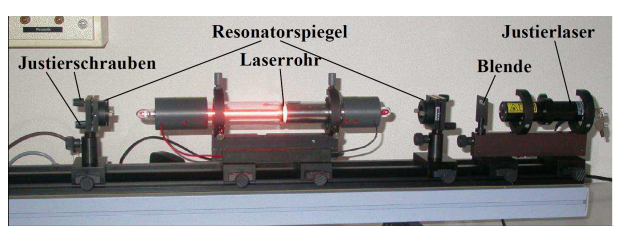
\includegraphics[scale=0.55]{fig/aufbauhene.png}
  \caption{Der verwendete Versuchsaufbau \cite{Anleitung1}}
  \label{fig:aufbauhene}
\end{figure}
Der Versuchsaufbau besteht wie in Abbildung (\ref{fig:aufbauhene}) zu sehen aus einer optischen Schiene auf der ein Laserrohr, zwei Spiegel, Blenden sowie ein Laser zum Justieren der Apparatur befestigt sind. Die geometrischen Daten
des mit einem Helium-Neon-Gasgemisch gefüllten Laserrohr sind gegeben durch die Länge $L=\SI{408}{\milli\meter}$ sowie den Durchmesser $d_\mathrm{HeNe}=\SI{1.1}{\milli\meter}$. Das Laserrohr ist außerdem mit Elektroden versehen die durch Entladung die Besetzungsinversion auslösen. Desweiteren ist das Laserrohr mit den in Abschnitt (\ref{sec:brews}) beschriebenen Brewsterfenstern abgeschlossen. In Tabelle (\ref{tab:spiegel}) sind die verfügbaren Spiegel aufgelistet.
\begin{table}
  \centering
  \caption{Die Daten der verfügbaren Spiegel}
  \label{tab:spiegel}
  \begin{tabular}{c | c | c}
    \toprule
    Spiegel & Bezeichnung & Oberflächenbeschaffenheit \\
    \midrule
    plan & flat/flat & HR (high reflectivity) $R \geq 99\%$ \\
    konkav & $r=\SI{1000}{\milli\meter}$/flat & HR (high reflectivity) $R \geq 99\%$ \\
    konkav & $r=\SI{1400}{\milli\meter}$/flat & HR (high reflectivity) $R \geq 99\%$ \\
    konkav & $r=\SI{1400}{\milli\meter}$/flat & OC (out coupling) $T=1.5-1.8\%$ \\
    \bottomrule
  \end{tabular}
\end{table}
Damit der HeNe-Laser justiert werden kann befindet sich der Justier-Laser auf der optischen Schiene mit der Wellenlänge $\lambda=\SI{532}{\nano\meter}$, der maximalen Leistung $P_\mathrm{max}=\SI{1}{\milli\watt}$ sowie der für die Justage verwendeten reduzierten Leistung $P_\mathrm{grün}=\SI{0.2}{\milli\watt}$.
\subsection{Durchführung}
\label{sec:durchff}
Die Messungen wurden in der folgenden Reihenfolge durchgeführt. Für die Messungen der $\mathrm{TEM}$-Moden, der Polarisation des Lasers und der Bestimmung der Wellenlänge wurden die Spiegel 3 und 4 aus Tabelle (\ref{tab:spiegel}) benutzt. Dies entspricht Anordnung 1 aus Abbildung (\ref{fig:plot1}).
Die Spiegel befanden sich dabei im Abstand von $L=\SI{72}{\centi\meter}$, da so die Intensitätsschwankungen am Geringsten waren.
\subsubsection{Justierung des He-Ne-Lasers}
Für die Justage des He-Ne-Lasers werden mithilfe des Justierungslasers die Resonatorspiegel und das Laserrohr so eingestellt, dass der Laserstrahl mittig auf die Justierblende fällt, dafür wird ein Fadenkreuz verwendet.
Nach dieser Justage kann der Versuch beginnen. Während des eigentlichen Experimentes ist der Justierungslaser ausgeschaltet.
\subsubsection{Überprüfung der Stabilitätsbedingung}
Nach der Justage wird nun als erstes die Stabilitätsbedingung überprüft, dafür wird zunächst der Laser auf maximale Leistung eingestellt und anschließend wird eine Messreihe der Intensität des Laserstrahls in Abhängigkeit von
der Resonatorlänge aufgenommen. Dabei ist eine Nachjustierung der Leistung bei Verschiebung der Resonatorspiegel notwendig. Die Messung wird für einen konkav-konkav und einen plan-konkav Resonator durchgeführt.
\subsubsection{TEM-Moden}
Zur Untersuchung der transversalen Moden $\mathrm{TEM}_\mathrm{00}$ und $\mathrm{TEM}_\mathrm{01}$ wird mithilfe einer Streulinse der Laserstrahl aufgefächert und anschließend auf eine Photodiode geleitet.
Die Intensitätsverteilung wird direkt von dieser mit einer Skala versehenen Diode abgelesen. Da die Grundmode $\mathrm{TEM}_\mathrm{00}$ wie in Abschnitt (\ref{sec:modee}) beschrieben den größten Anteil am Modenspektrum besitzt kann
diese ohne weiteres Justieren der Apparatur vermessen werden. Damit die Mode $\mathrm{TEM}_\mathrm{01}$ sichtbar wird, wird das Laserrohr leicht justiert.
\subsubsection{Polarisation des Lasers}
\label{sec:polari}
Um die Polarisation des Lasers zu bestimmen wird eine Messreihe mit einem Polarisationsfilter aufgenommen. Dafür wird dieser von $\SI{0}{\degree}$ bis $\SI{180}{\degree}$ im Strahlengang variiert und die Intensität in Abhängigkeit von der Polarisation des Filter wieder mithilfe einer Photodiode gemessen.
\subsubsection{Wellenlänge des Lasers}
Im letzten Teil der Durchführung soll nun mithilfe eines Gitters die Wellenlänge des Lasers bestimmt werden. Dafür wird ein Schirm auf den der Laserstrahl projeziert wird in einem hinreichend großen Abstand hinter das Gitter gestellt, sodass nulltes und die beiden ersten Maxima zu sehen sind. Dann werden die Abstände zwischen nulltem und ersten Maxima, Gitterkonstante sowie der Abstand zwischen Gitter und Schirm aufgeschrieben.
